\documentclass[12pt]{article}

\usepackage{tabularx}
\usepackage[a4paper,margin=2.5cm, bottom=4cm]{geometry}
\usepackage{fancyhdr}
\usepackage{listings}
\usepackage{booktabs}
\usepackage{float}
\usepackage{subcaption}
\usepackage{graphicx}
\usepackage{amsmath}
\usepackage{amssymb}
\usepackage[table]{xcolor}
\usepackage{pgfplots}
\usepackage{tikz}
\pgfplotsset{compat=1.17}

\graphicspath{{../img/}}

\setlength{\headheight}{40pt}
\setlength{\parindent}{0pt}
\setlength{\parskip}{1ex}
\renewcommand{\headrulewidth}{0pt}

\newcommand{\subfiguresize}{.3\textwidth}

\lstset {
    basicstyle = \small\ttfamily,
}

\begin{document}

\pagestyle{fancy}
\fancyhead{}
\fancyhead[L]{
    \renewcommand{\arraystretch}{1.5}
    \begin{tabularx}{\textwidth}{|X|X|}
        \hline
        \large \bf Image processing & \normalsize Task No. 1 \\
        \hline
    \end{tabularx}
}
\fancyfoot[C]{\thepage}

\thispagestyle{empty}
\renewcommand{\arraystretch}{2}
\begin{flushleft}
    \begin{tabularx}{0.95\textwidth}{|X|X|}
        \hline
        \bf \large Image Processing                   & \bf \large Task No.~1                           \\ \hline
        \multicolumn{2}{|l|}{
            \textbf{Task variant:} Group 1
        }                                                                                               \\ \hline
        \textbf{Day and time:} Mon, 14:00             & \textbf{Full name:} \textsc{Jakub Pawlak}       \\
        \textbf{Academic year: 3\textsuperscript{rd}} & \textbf{Full name:} \textsc{Magdalena Paku\l a} \\
        \hline
    \end{tabularx}
\end{flushleft}
\vspace{1em}
\renewcommand{\arraystretch}{1}

\section{Technical description of the program}
\subsection{Basic information}

Technical description of the application
This application allows a user to apply some operations to bitmap files, which are:
\begin{enumerate}
    \item basic color correction operations such as modifying brightness or contrast
    \item geometric operations, for example resizing or flipping the image
    \item noise removal filters (in this case median and geometric mean)
\end{enumerate}
We decided to write our project in the Rust programming language due to its multiple advantages, such as:
high speed due to it being compiled language like C++, yet with much more safety mechanisms for managing memory without the use of a garbage collector.

To view the instructions of usage, the user should invoke the program with ``\lstinline{--help}'' argument.
This will print all of the available operations, including the arguments that the user should provide.
The basic format for all the operations are:
\begin{center}
    \lstinline{executable --command [-argument=value]* input_file}
\end{center}

\subsection{Advanced information}
\subsubsection{Used libraries}
The external libraries (called ``crates'' in case of Rust) that we use in our project are
\begin{itemize}
    \item \textbf{image} --- providing implementations of image encoders and decoders,
          used for reading and saving the images
    \item \textbf{vulkano} --- Rust wrapper around the Vulkan graphical API,
          which we use to provide alternative implementations of some transformations,
          which are run on the GPU making them significantly faster
    \item \textbf{vulkano-shaders} --- providing some macros that automatically,
          during the program's compilation,
          also compile the glsl shader code and embed it in the final binary.
\end{itemize}

\subsubsection{Data structures}
For storing the image we use RgbImage struct from the mentioned image crate,
which is just a wrapper around a vector of pixels, which in turn are just a 3-element array of unsigned 8-bit integers (one for each RGB channel).

\section{Description of implementation of basic image operations}

\paragraph*{Preface on the used notation}
In the equations we write to describe operations, we will use luminosity functions $f$ to describe the original image, and $\hat{f}$ to describe the new image (after transformation).
$f(x,y)$ will denote the luminosity of the pixel at the coordinates $x,y$. Unless explicitly stated, the method will be the same for each color channel.
For brevity, if the pixel coordinates are irrelevant, they may be ommited and be assumed to be the same for $\hat{f}$ and $f$, i.e.\ $\hat{f}=f$ is equivalent to $\hat{f}(x,y) = f(x,y)$.
Additionally, we define $x|_{[a,b]}$ as $x$ restricted to the range $[a,b]$, that is $\max\{a, \min\{x,b\}\}$.
For parameters that are specified by the user (e.g\ in brightness or contrast modifications), we will use letters from the greek alphabet.

\subsection{Brightness modification (B1)}

\subsubsection{Implementation}

For modyfying brightness we simply add the amount supplied by the user to the luminosity value of each pixel.
Because such operation can exceed the range of allowed values, we have to restrict the result to the range $[0,255]$.

\begin{equation}
    \hat{f} = (f + \alpha) \, \Big|_{[0,255]}
\end{equation}

\subsubsection{Results}

\begin{figure}[H]\centering
    \begin{subfigure}[t]{\subfiguresize}\centering
        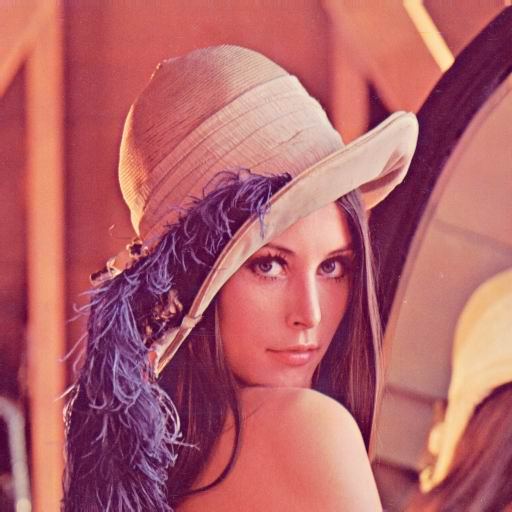
\includegraphics[width=\textwidth]{lenac.png}
        \caption{original}
    \end{subfigure}
    \hspace{.05\textwidth}
    \begin{subfigure}[t]{\subfiguresize}\centering
        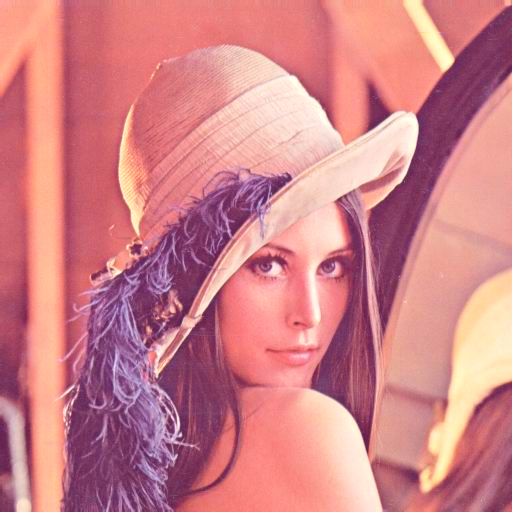
\includegraphics[width=\textwidth]{lenac_bright+30.png}
        \caption{with increased brightness}
    \end{subfigure}
    \caption{Image before and after increasing the brightness by 30}
\end{figure}

\subsubsection{Complexity analysis}

The operation for one pixel is of constant time,
therefore the total computational complexity for the image of size $w \times h$ is $\mathcal{O}(wh)$.
The algorithm operates in-place, therefore it's space complexity is $\mathcal{O}(1)$.

\subsection{Contrast modification (B2)}

\subsubsection{Implementation}

For contrast modification, we want to multiply the luminosity values by the specified factor
in order to modify the slope of the tone curve.

However, plain multiplication would result in visible brighness modification alogside the contrast change.
We, however, would like to make the dark pixels darker, and bright ones brighter.
For this reason, we offset the input luminosity by 128, to produce rotation around the center.

\begin{figure}[ht]\centering
    \begin{tikzpicture}
        \begin{axis}[
                % width=.5\textwidth,
                height = .4\textwidth,
                xmin=0,
                xmax=255,
                ymin=0,
                ymax=255,
                xtick = {0,255},
                xlabel = {\small input},
                ytick = {0,255},
                ylabel = {\small output}
            ]
            \addplot[black,domain=0:255,dotted]{x};
            \addplot[blue,domain=0:255,thick]{min(x*2,254)};
            \addplot[red,domain=0:255,thick]{max(1,min((x-128)*2+128,254))};
            % should be clamped to [0,255], but we use [1,254] for better visibility
        \end{axis}
    \end{tikzpicture}
    \caption{Contrast modification ($\alpha = 2$) without offset (blue), and with offset (red)}
    \label{fig:contrast-differences}
\end{figure}

The difference is shown of fig. \ref{fig:contrast-differences}.
We can clearly see the benefit of using the offset, so for computation we will use the following formula:

\begin{equation}
    \hat{f} = \left((f - 128) \cdot \alpha + 128\right)\Big|_{[0,255]}
\end{equation}

\subsubsection{Results}

\begin{figure}[H]\centering
    \begin{subfigure}[t]{\subfiguresize}\centering
        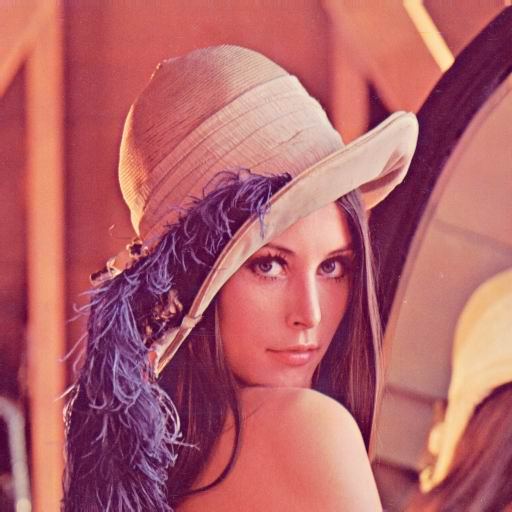
\includegraphics[width=\textwidth]{lenac.png}
        \caption{original}
    \end{subfigure}
    \hspace{.05\textwidth}
    \begin{subfigure}[t]{\subfiguresize}\centering
        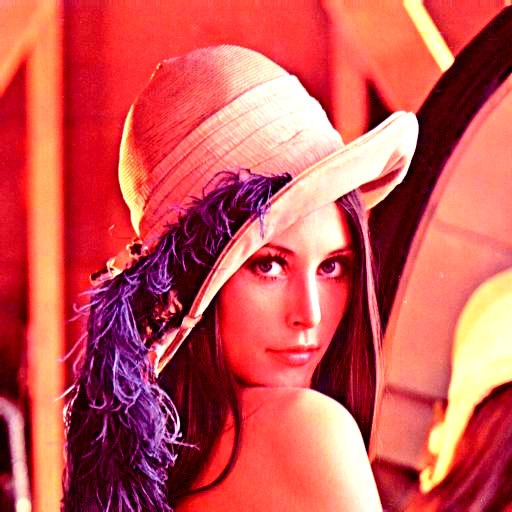
\includegraphics[width=\textwidth]{lenac_contrast_2x.png}
        \caption{with increased contrast}
    \end{subfigure}
    \caption{Image before and after increasing the contrast by a factor of 2}
\end{figure}

\subsubsection{Complexity analysis}

The operation for one pixel is of constant time,
therefore the total computational complexity for the image of size $w \times h$ is $\mathcal{O}(wh)$.
The algorithm operates in-place, therefore it's space complexity is $\mathcal{O}(1)$.

\subsection{Negative (B3)}

\subsubsection{Implementation}

Negative is produced by subtracting each pixel from the maximum intensity value, resulting in a complementary color.
It can be expressed as the following equation:

\begin{equation}
    \hat{f} = 255 - f
\end{equation}

\subsubsection{Results}

\begin{figure}[H]\centering
    \begin{subfigure}[t]{\subfiguresize}\centering
        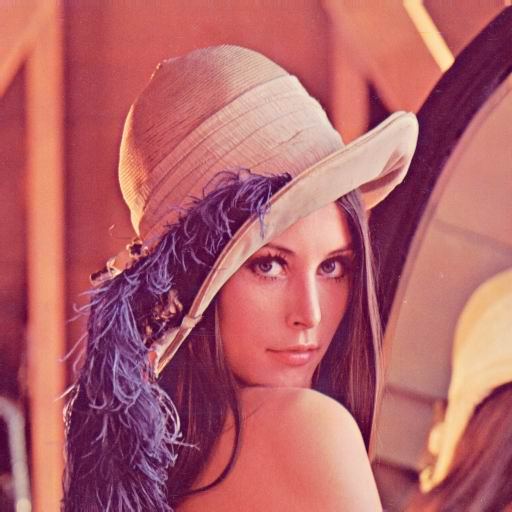
\includegraphics[width=\textwidth]{lenac.png}
        \caption{original}
    \end{subfigure}
    \hspace{.05\textwidth}
    \begin{subfigure}[t]{\subfiguresize}\centering
        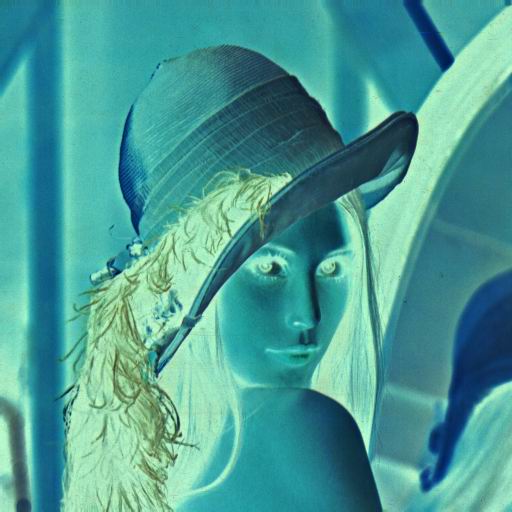
\includegraphics[width=\textwidth]{lenac_negative.png}
        \caption{negative}
    \end{subfigure}
    \caption{Image before and after inverting the colors}
\end{figure}

\subsubsection{Complexity analysis}

The operation for one pair of pixex is of constant time,
therefore the total computational complexity for the image of size $w \times h$ is $\mathcal{O}(\frac{wh}{2}) = \mathcal{O}(wh)$.
The algorithm operates in-place, therefore it's space complexity is $\mathcal{O}(1)$.

\subsection{Horizontal flip (G1)}

\subsubsection{Implementation}

Horizontal flip performs a mirroring operation around the vertical axis.
Therefore, the $y$ coordinates will remain unchanged, and $x$ coordinates will be mirrored around the center.
\begin{equation}
    \hat{f}(x,y) = f(width - x, y)
\end{equation}

We accomplish this by looping over every pixel in the left half of the image,
and swapping it with it's mirror pixel.

We loop only over the left half
because otherwise, each pair of pixels would be swapped twice,
cancelling each other.

\subsubsection{Results}

\begin{figure}[H]\centering
    \begin{subfigure}[t]{\subfiguresize}\centering
        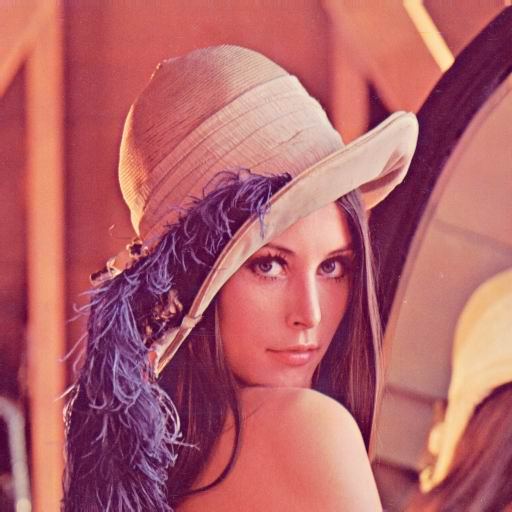
\includegraphics[width=\textwidth]{lenac.png}
        \caption{original}
    \end{subfigure}
    \hspace{.05\textwidth}
    \begin{subfigure}[t]{\subfiguresize}\centering
        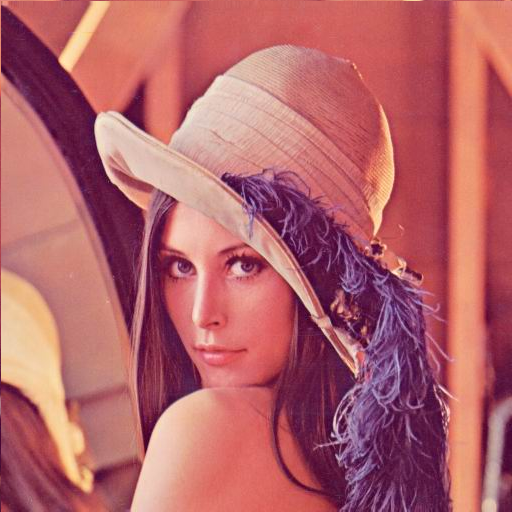
\includegraphics[width=\textwidth]{lenac_hflip.png}
        \caption{flipped}
    \end{subfigure}
    \caption{Image before and after flipping it horizontally}
\end{figure}

\subsubsection{Complexity analysis}



\subsection{Vertical flip (G2)}

\begin{equation}
    \hat{f}(x,y) = f(x, height - y)
\end{equation}

\begin{figure}[H]\centering
    \begin{subfigure}[t]{\subfiguresize}\centering
        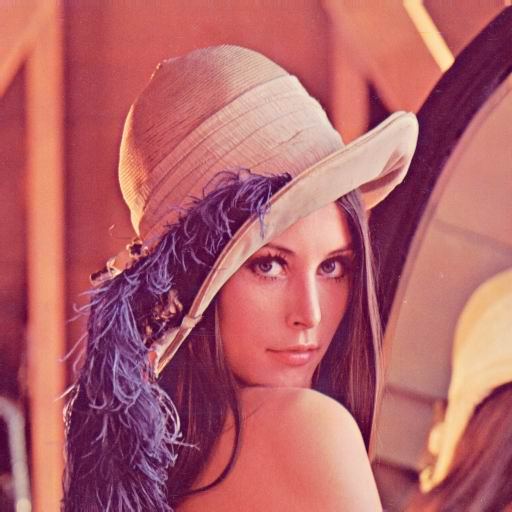
\includegraphics[width=\textwidth]{lenac.png}
        \caption{original}
    \end{subfigure}
    \hspace{.05\textwidth}
    \begin{subfigure}[t]{\subfiguresize}\centering
        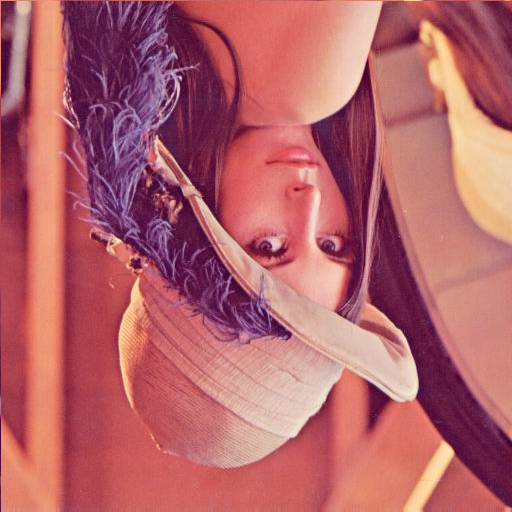
\includegraphics[width=\textwidth]{lenac_vflip.png}
        \caption{flipped}
    \end{subfigure}
    \caption{Image before and after flipping it vertically}
\end{figure}

\subsection{Diagonal flip (G3)}

\begin{equation}
    \hat{f}(x,y) = f(width - x, height - y)
\end{equation}

\begin{figure}[H]\centering
    \begin{subfigure}[t]{\subfiguresize}\centering
        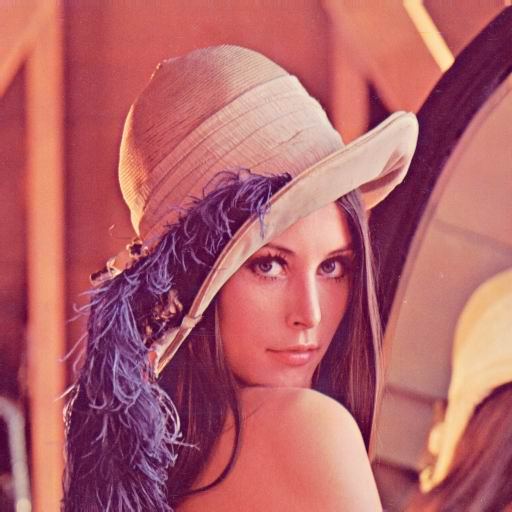
\includegraphics[width=\textwidth]{lenac.png}
        \caption{original}
    \end{subfigure}
    \hspace{.05\textwidth}
    \begin{subfigure}[t]{\subfiguresize}\centering
        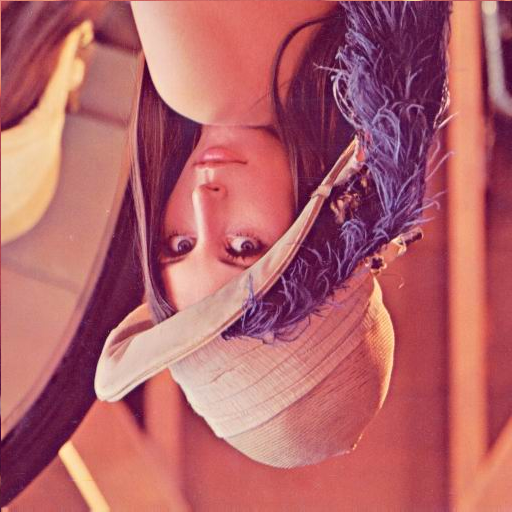
\includegraphics[width=\textwidth]{lenac_dflip.png}
        \caption{flipped}
    \end{subfigure}
    \caption{Image before and after flipping it diagonally}
\end{figure}

\subsection{Shrink (G4) and Enlarge (G5)}

For shrinking and enlarging, we will implement just one transformation, called scale.
Given some factors $\varphi_x, \varphi_y$ and an image with dimensions $w \times h$, it will produce a new image of dimensions $\varphi_x w \times \varphi_y h$.

\begin{equation}
    \hat{f}(x,y) =
    f\left(
    \left\lfloor
    \frac{x}{\varphi_x}
    \right\rfloor,
    \left\lfloor
    \frac{y}{\varphi_y}
    \right\rfloor
    \right)
\end{equation}

Although our function allows for different scaling factors
in the $x$ and $y$ dimensions,
the user is only able to input one value $\varphi$,
to preserve the original image aspect ratio,
so the program just sets $\varphi_x = \varphi_y = \varphi$.

Enlarge will just apply scale with the factor as it is, and shrink will apply scale, but with the inverse of the specified factor,
i.e.\ if we want to shrink by a factor of 2, we will apply scale with a factor of $\frac{1}{2}$.

\begin{figure}[H]\centering
    \begin{subfigure}[t]{\subfiguresize}\centering
        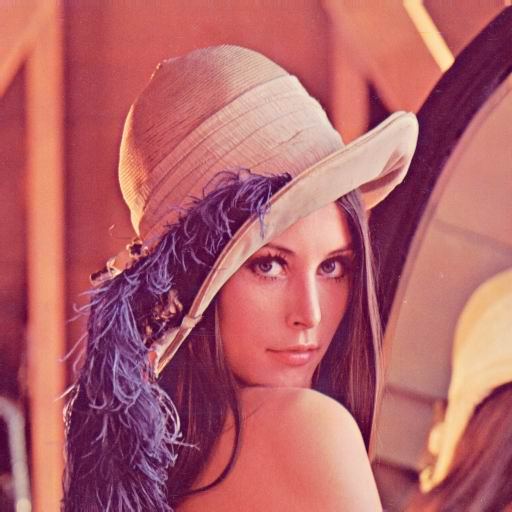
\includegraphics[width=\textwidth]{lenac.png}
        \caption{original ($512 \times 512$)}
    \end{subfigure}
    \hspace{.05\textwidth}
    \begin{subfigure}[t]{\subfiguresize}\centering
        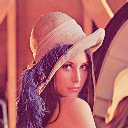
\includegraphics[width=.7\textwidth]{lenac_small.png}
        \caption{shrunk ($128 \times 128$)}
    \end{subfigure}
    \caption{Image before and after shrinking by a factor of 4 (not to scale)}
\end{figure}

\begin{figure}[H]\centering
    \begin{subfigure}[t]{\subfiguresize}\centering
        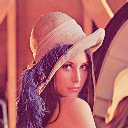
\includegraphics[width=.7\textwidth]{lenac_small.png}
        \caption{original ($128 \times 128$)}
    \end{subfigure}
    \hspace{.05\textwidth}
    \begin{subfigure}[t]{\subfiguresize}\centering
        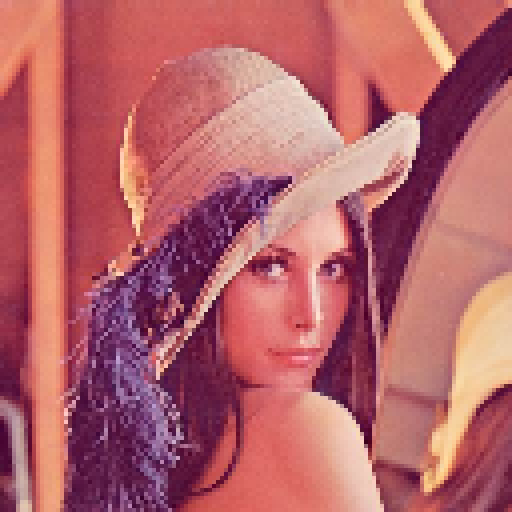
\includegraphics[width=\textwidth]{lenac_enlarged.png}
        \caption{enlarged ($512 \times 512$)}
    \end{subfigure}
    \caption{Image before and after enlarging by a factor of 4 (not to scale)}
\end{figure}

\section{Description of the implementation of the noise reduction methods}

\subsection*{Common implementation}
We noticed that all the filters operate by gathering some neighbourhood around the target pixel,
and then applying some reducing function on that pixels to determine the value of the resulting pixel.
Therefore, in order to remove duplication, we extracted the common functionality of gathering the pixels to a separate function $collect\_pixels$, such that:

\begin{equation*}
    collect\_pixels : \mathbf{Ref}\langle\mathrm{Image}\rangle \times \mathbb{N}^4 \to \mathbf{Vec}\langle \mathbf{Ref}\langle\mathrm{Pixel} \rangle\rangle
\end{equation*}

Note that we return the pixels by read-only reference, so we are not performing unnecessary copies.

Let $Img$ denote some image, and $Img_{(x,y)}$ the pixel of $Img$ at coordinates $x,y$.
Let $w$ and $h$ be width and height of $Img$.
Then, $collect\_pixels(Img,x,y,r_x,r_y)$ will return the pixels of $Img$ in some neighbourhood $S_{(x,y)}$ around $(x,y)$, defined as follows:
\begin{equation}
    S_{(x,y)} =
    \\\bigg\{
    Img_{(x,y)} \mid x \in [x-r_x,x+r_x] \cap [0,w) \land y \in [y-r_y, y+r_y] \cap [0,h)
    \bigg\}
\end{equation}

\subsection{Median filter (N1)}

\subsubsection{Implementation}\label{sec:median-impl}

The median filter works very simply, it just picks the median luminosity from the neighbourhood.

\begin{equation}
    \hat{f}(x,y) = \mathrm{median} \big\{ S_{(x,y)} \big\}
\end{equation}

While we could sort the values, and then pick the middle one,
we found the sorting to be problematic, as many sorting algorithms cannot go below $\mathcal{O}(n \log n)$.
For this reason, we used a more optimal approach, allowing as to get the median in $\mathcal{O}(n)$ time.

We define a sequence $(L_n)_{n=0}^{255}$, such that $L_n = n\big(\{p \in S_{(x,y)} \mid \mathrm{luminosity}(p) = n\}\big)$.

For example $L_{128}$ will be the number of pixels that have the luminosity 128.

From this sequence, finding the median is trivial, it is just $\mathbf{min}\big\{n \mid \sum_{k=0}^n L_k > \lfloor n(S)/2 \rfloor \big\}$

\paragraph*{Example\\}
Consider the neighbourhood $S = \{1,1,1,2,4,5,6\}$.
Then, our bucket array will look like this:
\begin{table}[H]\centering
    \begin{tabular}{|r|c|c|c|c|c|c|c|}
        \hline
        $\phantom{\big|}n$                & 0 & 1 & 2 & 3 & 4 & 5 & 6 \\ \hline
        $\phantom{\big|}L_n$              & 0 & 3 & 1 & 0 & 1 & 1 & 1 \\ \hline\hline
        $\phantom{\Big|}\sum_{k=0}^n L_k$ & 0 & 3 & 4 & 4 & 5 & 6 & 7 \\
        \hline
    \end{tabular}
\end{table}

Since $n(S) = 7$, the median index will be $\lfloor 7/2 \rfloor = 3$.
The first partial sum greater than 3 is 4, with index 2. Therefore, our median is 2.

\subsubsection{Complexity analysis}

Let $w,h$ be the dimensions of the image, and $m,n$, the dimensions of the sampling region (the neighbourhood).
For each pixel, i.e.\ $wh$ times, we must calculate the median, which takes $\mathcal{O}(mn)$.
Therefore, the total computational complexity is $\mathcal{O}(whmn)$.

In terms of space complexity, since our computation operates on not one pixel, but a neighbourhood, we must avoid corrupting the state.
We cannot perform the operation in-place, but rather must create a second image buffer.
Therefore the spacial complexity of the median filter is $\mathcal{O}(wh)$.

\subsection{GPU-accelerated Median filter}

Since filtering the image is computationally intensive, we decided to implement it also on the \textsc{gpu}.
We took advantage of it's parallel processing capabilities to \emph{significantly} improve the execution time.

\subsubsection{Implementation}\label{sec:median-gpu-impl}

To interface with the \textsc{gpu} we decided to use Vulkan API,
and ``vulkano'' crate as a wraper for interfacing with Rust.
To eliminate the tedious and repetitive parts of performing the calculations on the \textsc{gpu},
we wrote a helper struct --- \lstinline{InOutImageTransformationPipeline}.
This struct takes care of setting up the environment for transformations that take image as an input and produce an image as the output.
It's responsibilities are to create image views and buffers, binding them to the descriptor sets, and configuring the command buffer from a shader supplied in the constructor.

The shader code is semantically identical to the \textsc{cpu} version ---
we loop the neighbourhood and calculate the median luminance in the same way as described in section \ref{sec:median-impl}.
In the shader we use work group size of $16\times16$ --- a standard size when it comes to image processing.
The important thing is that we must pass the size of the neighbourhood to the shader.
We accomplish that by using push constant that contain values of $r_x$ and $r_y$.

In Rust code, we invoke the \lstinline{vulkano_shaders::shader!} macro, that compiles the shader source code and generates the struct for push constants.
Then, we set appropriate values in the push constants struct, and create the abovementioned transformation pipeline,
passing it the compiled shader, push constants, and gropup counts, which are calculated as $w / 16 + 1$ and $h / 16 + 1$ for $x$ and $y$ directions respectively.
(Note that we must add one to avoid black strips in case the image dimensions are not divisible by 16).

\subsubsection{Complexity analysis}

Calculating the standard computational complexity is not a very good measure for calculations performed on the \textsc{gpu},
so instead, we will calculate the work~($T_1$), and span~($T_\infty$) which are measures that take into account the parrallelization of work.

Work is the complexity in a single-threaded scenario, and in this case it is equal to the complexity of the \textsc{cpu}-based implementation of the median filter: $T_1 = \mathcal{O}(whmn)$. 
The span is the complexity assuming perfect parrallelism of all the computations.
In this case all of the work groups will execute simultaneously, so, since the work group size is constant, 
the span will depend only on the dimensions of the sampling region.
Therefore $T_\infty = \mathcal{O}(mn)$.

The space complexity will be the same as in the \textsc{cpu} implementation --- $\mathcal{O}(wh)$.
\end{document}